\documentclass[paper=a4, fontsize=18pt]{article} % A4 paper and 11pt font size
\usepackage{lmodern}
\usepackage[T1]{fontenc} % Use 8-bit encoding that has 256 glyphs
\usepackage{graphicx}
\usepackage{epstopdf}
\usepackage{subfigure}
%\usepackage{fourier} % Use the Adobe Utopia font for the document - comment this line to return to the LaTeX default
\usepackage[english]{babel} % English language/hyphenation
\usepackage{amsmath,amsfonts,amsthm} % Math packages
\usepackage[linesnumbered,ruled,vlined]{algorithm2e}
\usepackage{lipsum} % Used for inserting dummy 'Lorem ipsum' text into the template
\usepackage{sectsty} % Allows customizing section commands
\usepackage{hyperref}
%\allsectionsfont{\centering \normalfont\scshape} % Make all sections centered, the default font and small caps
\usepackage{fancyhdr} % Custom headers and footers
\usepackage{multirow}
\usepackage{pdfpages}
\usepackage[DIV12,pagesize]{typearea}
%\usepackage{multicolumn}
\pagestyle{fancyplain} % Makes all pages in the document conform to the custom headers and footers
\fancyhead{} % No page header - if you want one, create it in the same way as the footers below
\fancyfoot[L]{} % Empty left footer
\fancyfoot[C]{} % Empty center footer
\fancyfoot[R]{\thepage} % Page numbering for right footer
\renewcommand{\headrulewidth}{0pt} % Remove header underlines
\renewcommand{\footrulewidth}{0pt} % Remove footer underlines
\setlength{\headheight}{13.6pt} % Customize the height of the header
\setlength{\parskip}{0.5\baselineskip}

\numberwithin{equation}{section} % Number equations within sections (i.e. 1.1, 1.2, 2.1, 2.2 instead of 1, 2, 3, 4)
\numberwithin{figure}{section} % Number figures within sections (i.e. 1.1, 1.2, 2.1, 2.2 instead of 1, 2, 3, 4)
\numberwithin{table}{section} % Number tables within sections (i.e. 1.1, 1.2, 2.1, 2.2 instead of 1, 2, 3, 4)

\newcommand{\mM}{\mathcal{M}}
\newcommand{\mL}{\mathcal{L}}
\newcommand{\mB}{\mathcal{B}}
\newcommand{\mT}{\mathcal{T}}
\newcommand{\mS}{\mathcal{S}}
\newcommand{\mP}{\mathcal{P}}
\newcommand{\mC}{\mathcal{C}}
\newcommand{\bH}{\mathbb{H}}

\setlength\parindent{0pt} % Removes all indentation from paragraphs - comment this line for an assignment with lots of text

\graphicspath{{pic/}}

%----------------------------------------------------------------------------------------
%	TITLE SECTION
%----------------------------------------------------------------------------------------
\newtheorem{definition}{Definition}{\itshape}{\rmfamily}
\newtheorem{theorem}{Theorem}{\itshape}{\rmfamily}
\newtheorem{corollary}{Corollary}{\itshape}{\rmfamily}
\newtheorem{example}{Example}{\itshape}{\rmfamily}
\newtheorem{proposition}{Proposition}{\itshape}{\rmfamily}
\newcommand{\horrule}[1]{\rule{\linewidth}{#1}} % Create horizontal rule command with 1 argument of height

\title{	
\normalfont \normalsize
\horrule{0.5pt} \\[0.4cm] % Thin top horizontal rule
\huge Survey of Intelligent Chatbots and Conversational Interfaces \\ % The assignment title
\horrule{2pt} \\[0.5cm] % Thick bottom horizontal rule
}
\hypersetup{hidelinks}

\author{}


\begin{document}

\maketitle
\section*{}

\subsection{Three New Graphical Models for Statistical Language Modelling \cite{Mnih2007}}

This paper shows how real-valued distributed representations for words can be learned at the same time as learning a large set of stochastic binary hidden features that are used to predict the distributed representation of the next word from previous distributed representations. One of the proposed models significantly outperforms the best $n$-gram models.

The first model is called the \emph{Factored Restricted Boltzmann Machine Language Model (FRBM)}. Each word is represented using a real-valued feature vector of length $N_f$. Let $R$ be an $N_w \times N_f$ matrix with row $i$ being the feature vector for the $i$-th word. The \emph{joint energy} of a sequence of words $w_1, ..., w_n$ is defined as:
$$E(w_n, h; w_{1:n-1}) = -(\sum_{i=1}^n v_i^T R W_i)h.$$
Here matrix $W_i$ specifies the interaction between the vector of hidden variables and the feature vector.

The joint conditional distribution of the next word and the hidden configuration $h$ is defined in terms of the energy function as:
$$P(w_n, h | w_{1:n-1}) = \frac{1}{Z_c} \exp(-E(w_n,h; w_{1:n-1})),$$
where $Z_c$ is a context-dependent normalization term. The conditional distribution of the next word can be obtained by marginalizing over the hidden variables.
\begin{figure}
  \centering
  % Requires \usepackage{graphicx}
  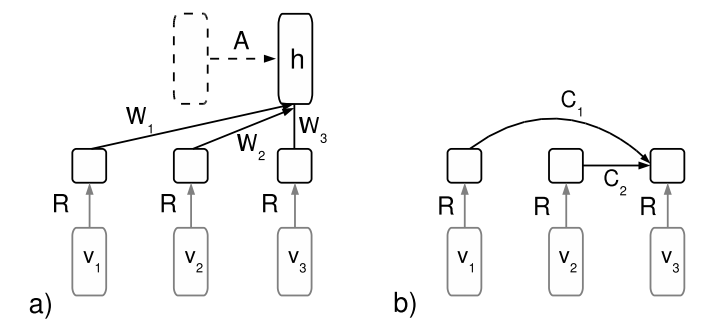
\includegraphics[width=.6\linewidth]{Minh07-RBM.png}\\
  \caption{a) The diagram for FRBM and TFRMB. The dashed part is included only for the TFRBM; b) The diagram for the log-bilinear model.}\label{fig:Minh07-RBM}
\end{figure}

The second model is called the \emph{Temporal Factored RBM (TFRBM)}. The basic idea is to make a simple extension to the factored RBM language model. Suppose we want to predict word $w_{t+n}$ from $w_1, ..., w_{t+n-1}$ for some large $t$. The method applies a separate instance of the model to words $w_\tau, ..., w_{\tau+n-1}$ for each $\tau$ in $\{1, ..., t\}$. In order to propagate context information forward, it further introduces directed connections from $h^\tau$ to $h^{\tau+1}$, and computes the hidden state of model $\tau+1$ using the inputs from the hidden state of model $\tau$ as well as its visible units. Figure \ref{fig:Minh07-RBM} (a) shows the diagram for the temporal FRBM.

The third model is called the \emph{log-bilinear language model}. The energy function of this model is specified as:
$$E(w_n; w_{1:n-1}) = -(\sum_{i=1}^{n-1} v_i^T R C_i)R^T v_n - b_r^T R^T v_n - b^T_v v_n.$$
In the FRBM energy function the interaction is between the word feature vectors and the hidden variables, whereas in this model the interaction is between the feature vectors for the context words and the feature vector for the predicted word. Intuitively, the model predicts a feature vector for the next word by computing a linear function of the context word feature vectors. Then it assigns probabilities to all words in the vocabulary based on the similarity. This model is similar to the energy-based model proposed in \cite{Bengio2003A}. However, the model proposed here uses a bilinear energy function, while the energy function in \cite{Bengio2003A} is a one-hidden-layer neural network. Figure \ref{fig:Minh07-RBM} (b) shows a diagram of the log-bilinear language model.

In the experimental study, the paper evaluates the proposed models using the \emph{Associated Press News (APNews)} dataset consisting of a text stream of about 16 million words. In the first experiment, it is shown that three of the four network models are competitive with $n$-gram models. The best results were obtained by averaging with the temporal network model, resulting in 21\% reduction in perplexity over the best $n$-gram model. In the second experiment, it is also shown that the log-bilinear models clearly outperform the $n$-gram models.

\subsection{Limited Domain Synthesis \cite{Black2000}}

This paper presents a reliable and efficient method for building limited domain speech synthesis voices. By constructing databases close to the target domain of the speech application, it uses \emph{unit selection} synthesis techniques to reliably give high quality synthesis within domain.

The task of building a voice consists of the following processes:
\begin{itemize}
\item{Design the corpus\\
The first step is to design a prompt list that adequately covers the domain. In general, prompts should have at least one occurrence of each word in the vocabulary in each prosodic context.
}
\item{Synthesize each utterance\\
The prompts are synthesized for a number of reasons: 1) ensure that all the tokens are expanded properly (e.g. flight numbers and dates); 2) estimate the time required for recording; 3) use the synthesized prompt in labeling the human spoken utterance.
}
\item{Record the voice talent\\
Recording with studio quality equipment gives better results, but the paper is also interested in making the process more accessible. It uses a laptop in a quiet room. The recording quality shows to be acceptable once audio devices are set up appropriately.
}
\item{Label the recordings\\
After recording, it labels the text using a simple but effective technique based on \cite{Malfrere1997}: it uses DTW to align between the mel-scale cepstral coefficients of the synthesized and recorded waveforms.
}
\item{Extract pitchmarks
}
\item{Extract pitch-synchronous parameters
}
\item{Build a cluster unit selection synthesizer\\
The unit selection technique used in this paper is an updated version of that more fully described in \cite{Black97}. The general algorithm takes all units of the same type and calculates an acoustic distance between each. Selected features including phonetic and prosodic context are used to build a decision tree that minimizes acoustic distance in each partition. At synthesis time, it selects the appropriate cluster using the decision tree, and then finds the best path through the candidates.
}
\item{Test and tune, repeating as necessary}
\end{itemize}

The proposed technique is tested on three domains: a talking clock, a weather report system, and the CMU Communicator system.

The original demonstration of this technique was a simple talking clock. The prompts consist of 24 simple utterances of the form: ``The time is now, a little after quarter past two in the afternoon.'' Not counting recording time, this takes around 3 minutes to build. Such clocks have also been built in languages other than English, such as Chinese.

The most difficult example is the CMU Communicator system. At first it appears that the domain is not closed, as it includes greeting to registered users by name, and allows reference to any airport in the world. For the words like cities and airports, which are essentially open classes, it used the frequency information in the logs to select which set to include in the recordings. For the more frequently mentioned cities it includes more than one occurrence in the prompts. The final voice was built in under one-man week. After the version was running, it made some changes to the language generation system, and constructed further 50 utterances and added them into the system in another morning's work.

\subsection{Multilingual Distributed Representations without Word Alignment \cite{Hermann2013}}

This paper proposes a method for learning distributed representations in a multiligual setup. The model learns to assign similar embeddings to aligned sentences and dissimilar ones to sentences which are not aligned. It shows that the representations are semantically informative and applies them to a cross-lingual document classification task.

The basic idea is that, given enough parallel data, a shared representation would be forced to capture the common elements between sentences from different languages. What two parallel sentences have in common, of course, is the semantics of those two sentences. Using such parallel data, it proposes a novel method for learning vector representations at the word level and beyond.

The first step is to define a bilingual error function as follows: given a \emph{compositional sentence model (CVM)} $\mM_A$, which maps a sentence to a vector, it trains a second CVM $\mM_B$ using a parallel corpus $\mC_{A,B}$. For each pair of parallel sentences $(a,b) \in \mC_{A,B}$, it attempts to minimize
$$E_{dist}(a,b) = ||a_{root} - b_{root}||^2,$$
where $a_{root}$ ($b_{root}$) is the vector representing sentence $a$ ($b$).

The CVM used in this paper is a simple additive composition function:
$$a_{root}= \sum_{i=0}^{|a|} a_i.$$
Due to the use of parallel data, we know that $a$ and $b$ are semantically equivalent. Hence the goal is to jointly train both models $\mM_A$ and $\mM_B$, so that
$$E_{bi}(\mC_{A,B}) = \sum_{(a,b) \in \mC_{A,B}} E_{dist}(a,b)$$
is minimized.

However, the models could learn to reduce all embeddings and composition weights to zeros and thereby minimize the objective function. This problem is addressed by penalizing small distances between non-parallel sentence pairs. For every pair of parallel sentences $(a,b)$ it samples a number of additional sentences $n \in \mC_B$, which are not exact translation of $a$:
$$E_{noise}(a, b, n) = [1 + E_{dist}(a,b) - E_{dist}(a,n)]_{+},$$
where $[x]_{+} = \max(x,0)$ denotes the standard hinge loss. Thus, the final objective function is defined to be:
$$J(\theta_{bi}) = \sum_{(a,b) \in \mC_{A,B}} (\sum_{i=1}^k E_{noise}(a,b,n_i)) + \frac{\lambda}{2} || \theta_{bi} ||^2.$$

\begin{figure}[h]
  \centering
  % Requires \usepackage{graphicx}
  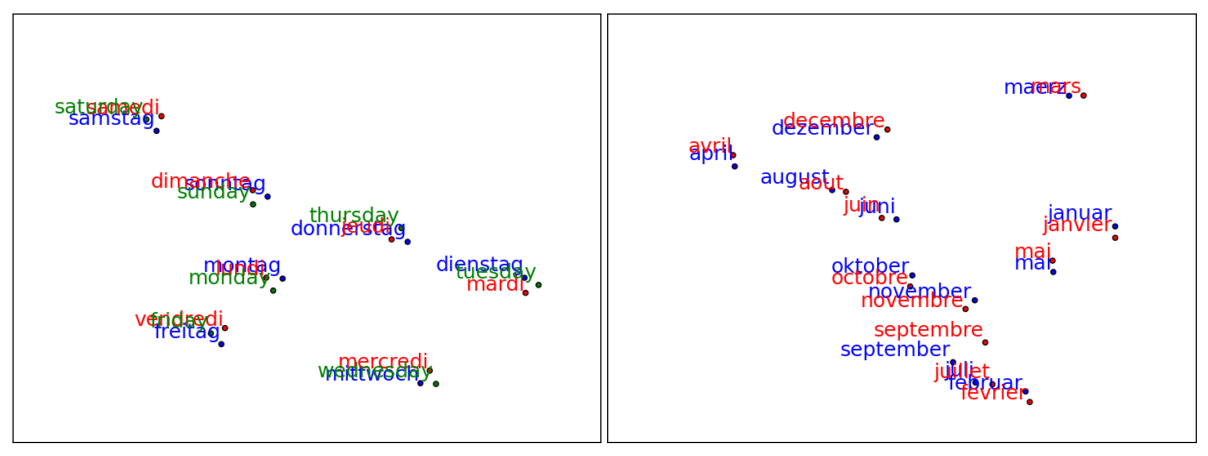
\includegraphics[width=\linewidth]{Hermann13-BiCVM.png}\\
  \caption{The left scatter plot shows t-SNE projections for a weekdays in three language. The right plots shows months using only the German and French words.}\label{fig:Hermann13-BiCVM}
\end{figure}

In the experimental study, the paper evaluates the proposed model in to experiments: the \emph{BiCVM} model was trained on 500k sentence pairs of a English-German parallel corpus. The \emph{BiCVM+} used this dataset in combination with anther 500k parallel sentences form the English-French section. The motivation behind BiCVM+ is to investigate whether it can learn better embeddings by introducing additional data in a different language. The models are evaluated on the \emph{cross-lingual document classification (CLDC)} task. It is shown that both models outperform all prior work on this task. Further, BiCVM+ outperforms BiCVM, indicating the usefulness of adding training data from a separate pair. Figure \ref{fig:Hermann13-BiCVM} shows the t-SNE projections for a number of English, French and German words.

\subsection{Energy-Based Models and Boltzmann Machines \cite{Bengio2009}}

In this survey we present the fifth chapter of the book \emph{Learning Deep Architectures for AI} by Bengio \cite{Bengio2009}. This chapter introduces the main mathematical concepts helpful to understand \emph{Restricted Boltzmann Machines (RBMs)}, which are particular energy-based models.

Energy-based models associate a scalar energy to each configuration of the variables of interest. For example, we would like plausible or desirable configurations to have low energy. The probability distribution of an energy-based model may be defined as follows:
\begin{equation}\label{equ:1}
P(x) = \frac{e^{-Energy(x)}}{Z}.
\end{equation}
Here $Z$ is a normalization term called the \emph{partition function} by analogy with physical systems.

In the \emph{products of experts} formulation, the energy function is a sum of terms, each one associated with an ``expert'' $f_i$:
\begin{equation}
Energy(x) = \sum_i f_i(x).
\end{equation}
Each expert can thus be seen as a detector of implausible configurations of $x$, or equivalently, as enforcing constraints on $x$.

In many cases we do not observe all the components simultaneously, or we want to introduce some non-observed variables to increase the expressive power of the model. So we consider an observed part $x$ and a hidden part $h$:
\begin{eqnarray}
P(x,h) = \frac{e^{-Energy(x,h)}}{Z},\\
P(x) = \sum_h P(x,h).
\end{eqnarray}
In order to map this formulation to the standard form, we introduce the notation of \emph{free energy}:
\begin{eqnarray}
P(x) = \frac{e^{-FreeEnergy(x)}}{Z},\\
FreeEnergy(x) = - \log \sum_h e^{-Energy(x,h)}.
\end{eqnarray}

The average log-likelihood gradient over the training set is
\begin{eqnarray}
E_{\hat{P}}[\frac{\partial \log P(x)}{\partial \theta}] = - E_{\hat{P}}[\frac{\partial FreeEnergy(x)}{\partial \theta}] + E_P[\frac{\partial FreeEnergy(x)}{\partial\theta}],
\end{eqnarray}
where expectations are over $x$, with $\hat{P}$ the training set empirical distribution and $E_P$ the expectation under the model's distribution.

If the energy can be written as a sum of terms associated with at most one hidden unit:
\begin{eqnarray}
Energy(x,h) = -\beta(x) + \sum_i \gamma_i(x, h_i),
\end{eqnarray}
then the free energy and numerator of the likelihood can be computed tractably:
\begin{eqnarray}
P(x) = \frac{e^\beta(x)}{Z} \prod_i \sum_{h_i} e^{-\gamma_i(x, h_i)}.
\end{eqnarray}

The \emph{Boltzmann machine} is a particular type of energy-based model with hidden variables. In a Boltzmann machine, the energy function is a general second-order polynomial:
\begin{eqnarray}
Energy(x,h) = -b'x - c'h - h'Wx - x'Ux - h'Vh.
\end{eqnarray}
The gradient of the log-likelihood can be written as:
\begin{eqnarray}
\frac{\partial \log P(x)}{\partial \theta} = - \sum_h P(h|x) \frac{\partial Energy(x,h)}{\partial \theta} + \sum_{\hat{x},h} P(\hat{x}, h) \frac{\partial Energy(\hat{x},h)}{\partial \theta}.
\end{eqnarray}
This gradient can be computed, if we have a procedure to sample from $P(h|x)$ and from $P(x,h)$. The basic idea is to use \emph{Gibbs sampling} in two phases: in the \emph{positive phase}, $x$ is clamped to the observed input vector, and we sample $h$ given $x$; in the \emph{negative phase} both $x$ and $h$ are sampled. Since two \emph{MCMCs (Monte Carlo Markov Chain)} (one for the positive phase and one for the negative phase) are needed for each example $x$, the computation can be very expensive.

\begin{figure}[h]
  \centering
  % Requires \usepackage{graphicx}
  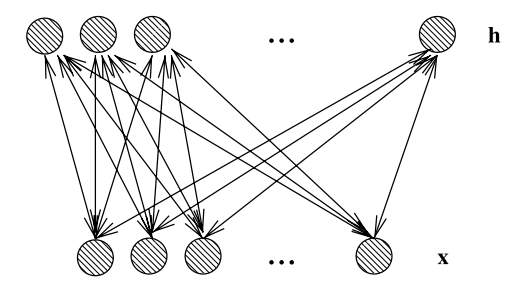
\includegraphics[width=.6\linewidth]{Bengio09-RBM.png}\\
  \caption{Undirected graphical model of a RBM}\label{fig:Bengio09}
\end{figure}

In the \emph{Restricted Boltzmann Machine (RBM)}, the $h_i$ are independent of each other when conditioning on $x$, and the $x_j$ are independent of each other when conditioning on $h$ (cf. Figure \ref{fig:Bengio09}). The energy function is bilinear:
\begin{eqnarray}
Energy(x,h) = -b'x - c'h - h'Wx.
\end{eqnarray}
The free energy of the input can be computed efficiently:
\begin{eqnarray}
FreeEnergy(x,h) = -b'x - \sum_i \log \sum_{h_i} e^{h_i(ci + W_i x)}.
\end{eqnarray}
Using the same factorization trick, we can obtain a tractable expression for $P(h|x)$ and $P(x|h)$.

Gibbs sampling in fully connected Boltzmann Machines is slow because there are as many sub-steps in the Gibbs chain as there are units in the network. The Factorization enjoyed by RBMs bring two benefits: 1) we do not need to sample in the positive phase because the free energy is computed analytically; 2) the set of variables $(x,h)$ can be sampled in two sub-steps in each step of the Gibbs chain: first we sample $h$ given $x$, and then a new $x$ given $h$.

\emph{Contrastive Divergence (CD)} is an approximation of the log-likelihood gradient that has been found to be a successful update rule for training RBMs. The basic idea of $k$-step CD is simple, and involves a second approximation, which introduces some bias in the gradient: run the MCMC chain $x_1, ..., x_{k+1}$ for only $k$ steps starting from the observed example $x_1 = x$. The surprising empirical result is that even $k=1$ often gives good results.


\subsection{Dialogue Act Modeling for Automatic Tagging and Recognition of Conversational Speech \cite{Stolcke2000}}

This paper describes a statistical approach for modeling \emph{dialogue acts (DAs)} on conversational speech, i.e., speech-act-like units such as \emph{Statement}, \emph{Question}, \emph{Backchannel}, etc. The proposed model detects and predicts dialogue acts based on lexical, collocational, and prosodic cues, as well as on the discourse coherence. It develops a probabilistic integration of speech recognition with dialogue modeling, to improve both speech recognition and dialogue act classification accuracy.

The goal of this paper is twofold: 1) presets a comprehensive framework for modeling and automatic classification of DAs, and proposes a framework that provides a mathematically principled way to condition the speech recognizer on conversation context through dialogue structure; 2) presents results obtained with this approach on a large, widely available corpus of spontaneous conversational speech.

This paper follows a recent standard for shallow discourse structure annotation, the \emph{Dialogue Act Markup in Several Layers (DAMSL)} tag set, which aims to provide a domain-independent framework for dialogue annotation.

The mathematical and computational framework used in the paper is the \emph{hidden Markov model (HMM)}. Given all available evidence $E$ about a conversation, the goal is to find the DA sequence $U$ that has the highest posterior probability $P(U|E)$ given that evidence.
$$U^* = \arg\max_U P(U|E) = \arg\max_U P(U) P(E|U).$$
Next we will discuss the prior probability $P(U)$, and the posterior probability $P(E|U)$ respectively.

In modelling the prior distribution $P(U)$, the paper assumes that the distribution is Markovian, i.e., each $U_i$ depends only on a fixed number $k$ of preceding DA labels:
$$P(U_i | U_1, ..., U_{i-1}) = P(U_i | U_{i-k}, ..., U_{i-1}).$$
The paper trains standard backoff N-gram models, using the frequency smoothing approach. The authors also tried several alternative approaches, but there was no significant improvement over the simple N-gram method.

The computation of $P(E|U)$ depends on the types of evidence use. The paper used the following three types of sources of evidence, either alone or in combination:
\begin{itemize}
\item{\textbf{Transcribed words}\\
$P(W|U)$, where $W$ refers to the true (hand-transcribed) words spoken in a conversation.
}
\item{\textbf{Recognized words}\\
A standard approach is to use the 1-best hypothesis. A more thorough approach is to compute $P(A|U)$ (where $A$ is the acoustics input) by decomposing it into an acoustic likelihood $P(A|W)$ and a word-based likelihood $P(W|U)$:
$$P(A|U) = \sum_W P(A|W) P(W|U).$$
}
\item{\textbf{Prosodic features}\\
$P(F|U)$, where $F$ are the features capturing various aspects of pitch, duration, energy, etc., of the speech signal. For the prosodic classifiers, the paper used CART-style decision trees. One example in the corpus was the distinction between backchannels and agreement. The prosodic tree trained on this task is shown in Figure \ref{fig:stolcke00-decision_tree}. The paper also tried to use neural network classifiers on this task, and tested
various network structures. However, there was no encouraging result.
\begin{figure}[h]
  \centering
  % Requires \usepackage{graphicx}
  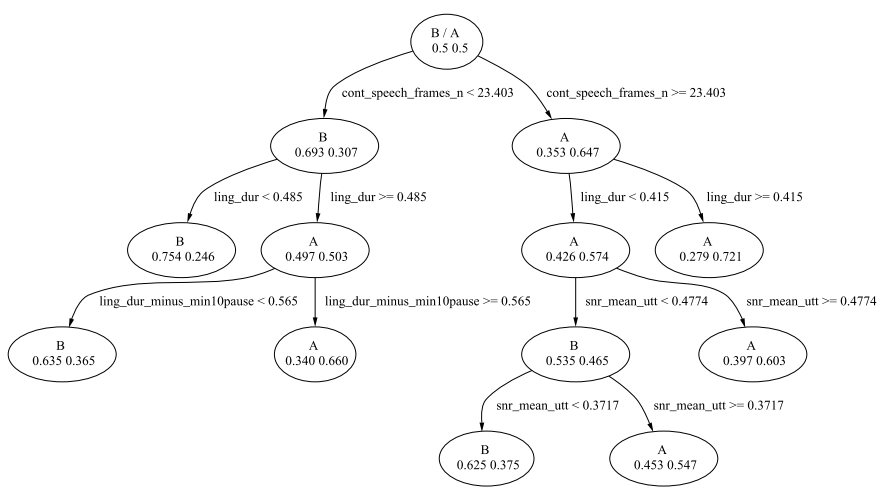
\includegraphics[width=\linewidth]{stolcke00-decision_tree.png}\\
  \caption{Decision tree for the classification of backchannels and agreements.}\label{fig:stolcke00-decision_tree}
\end{figure}
}
\end{itemize}

The paper proposes a method to combine multiple knowledge source, by using the following approximation:
\begin{align*}
P(A_i, W_i, F_i | U_i) &= P(A_i, W_i | U_i) P(F_i | A_i, W_i, U_i)\\
                       &\approx P(A_i, W_i | U_i) P(F_i | U_i).
\end{align*}

The HMM representation allows using efficient dynamic programming algorithms to compute relevant aspects of the model, such as: 1) the most probable DA sequence (the \emph{Viterbi algorithm}); 2) the posterior probability of various DAs for a given utterance (the \emph{forward-backward algorithm}).

The paper considers ways to use DA modeling to enhance automatic speech recognition (ASR). The first method is called \emph{mixture-of posteriors}, which yields:
$$P(W_i | A_i, E) = \sum_{U_i} \frac{P(W_i | U_i) P(A_i | W_i)}{P(A_i | U_i)} P(U_i | E).$$
The second method, called \emph{mixture-of-LM}, results in:
$$P(W_i | A_i, E) \approx (\sum_{U_i} P(W_i | U_i) P(U_i|E)) \frac{P(A_i |W_i)}{P(A_i)}.$$

The experiments confirmed that DA modeling can improve word recognition accuracy quite substantially in principle, at least for certain DA types.But the skewed distribution of DAs limits the usefulness of the approach on the Switchboard corpus. The paper suggests that the benefits of DA modeling might be more pronounced on corpora with more even DA distribution, which is typically the case for task-oriented dialogues.

\subsection{Recurrent Convolutional Neural Networks for Discourse Compositionality \cite{Kalchbrenner2013}}

This paper introduces both a sentence model and a discourse model corresponding to the two levels of compositionality: cords combine to form the meaning of sentences, and sentences combine to form the meaning of dialogues. The sentence model adopts convolution as the central operation, and is based on a novel \emph{hierarchical convolutional neural network (HCNN)}. The discourse model extends the sentence model, and is based on a \emph{recurrent neural network (RNN)}.

The basic kernel operation used in HCNN is described as follows. Given a sentence $s$ and its paired matrix $\mathbf{M}^s$, let $\mathbf{m}$ be a feature that is a row in $\mathbf{M}^s$. Let $w_1, ..., w_k$ be a sequence of $k$ weights. The local weighted addition over the first $k$ values is:
$$y = w_1 \mathbf{m}_1 + ... + w_k \mathbf{m}_k.$$
Then a kernel simply defines the value of $k$, and the one-dimensional convolution applies local weighted addition to each subsequence of values of $\mathbf{m}$. The one-dimensional convolution ($\mathbf{k} * \mathbf{m}$) is defined as:
$$(\mathbf{k} * \mathbf{m})_i = \sum_{j=1}^k \mathbf{k}_j \cdot \mathbf{m}_{k+i-j}.$$

To define the hierarchical architecture of the model, the paper next defines a sequence of kernel sizes and associated weights. Let $l$ be the number of words in the sentence $s$. The sequence of kernel sizes is defined as
$$k_1^l = 2, k_{i+1}^l = k_i^l + 1, k_t^l = l - \sum_{j=1}^{t-1}(k_j^l - 1).$$
That is, kernel sizes increase by one until the resulting convolved vector is smaller or equal to the last kernel size (cf. Figure \ref{fig:Kal13-hier}).

\begin{figure}[h]
  \centering
  % Requires \usepackage{graphicx}
  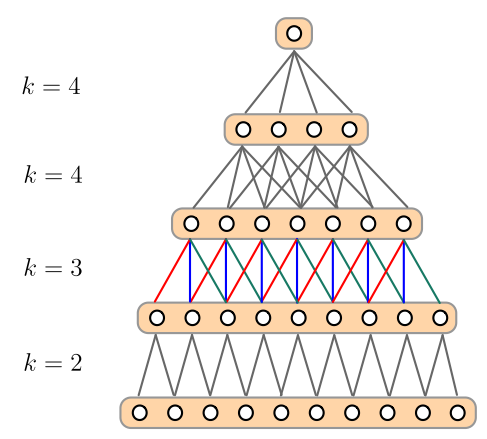
\includegraphics[width=.6\linewidth]{Kal13-hier_HCNN.png}\\
  \caption{A hierarchical convolutional neural network for sentential compositionality.}\label{fig:Kal13-hier}
\end{figure}

The composition operation in HCNN is formally defined as follows. For each feature $f$, let $\mathbf{K}_i^f$ be a sequence of $t$ kernels, where the size of the kernel $|\mathbf{K}_i^f| = k_i^l$. The hierarchy of matrices and corresponding features are defined as:
\begin{align*}
\mathbf{M}_{f,:}^1 &= \mathbf{M}_{f,:}^s,\\
\mathbf{M}_{f.:}^{i+1} &= \sigma(\mathbf{K}_i^f * \mathbf{M}_{f,:}^i + b_f^i).
\end{align*}

The discourse model adapts a RNN architecture in order to capture central properties of discourse. The proposed method aims to capture at least two of the most prominent properties: the sequentiality of the utterances, and the interactions between the speakers.

The RNN architecture takes inputs from a HCNN conditioned on the respective speakers. Let $s_1, ..., s_T$ be a sequence of sentences, each in turn being a sequence of words $s_i = y_1 ... y_l^i$. Let $x_1, ..., x_T$ be a sequence of labels, and $a_1, ..., a_T$ be a sequence of speaker. The RNN computes probability distribution by iterating the following equations:
\begin{align*}
\mathbf{h}_i &= \sigma(\mathbf{I} x_{i-1} + \mathbf{H}^{i-1}\mathbf{h}_{i-1} + \mathbf{Ss}_i + b_h)\\
         p_i &= softmax(\mathbf{O}^i \mathbf{h}_i + b_o)
\end{align*}

\begin{figure}[h]
  \centering
  % Requires \usepackage{graphicx}
  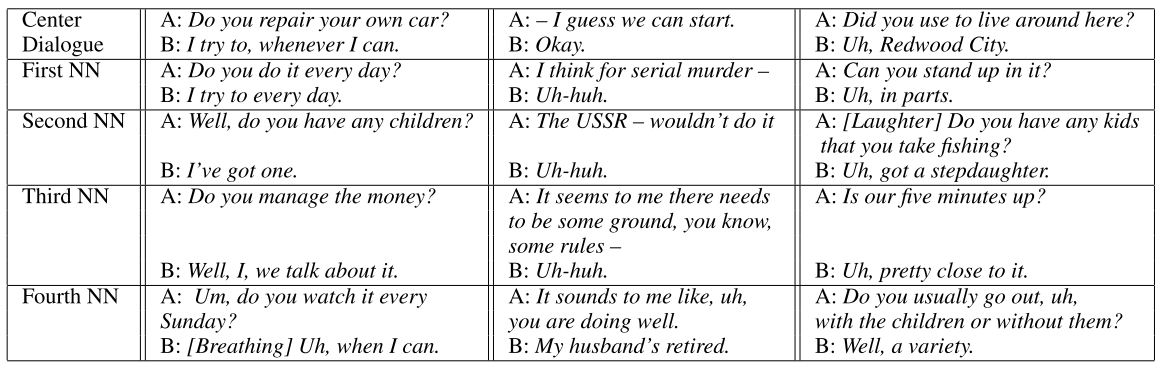
\includegraphics[width=\linewidth]{Kal13-NN.png}\\
  \caption{Short dialogues and nearest neighbours.}\label{fig:Kal13-NN}
\end{figure}

In the experimental study, the paper evaluates the proposed model with the prediction of dialogue acts within the \emph{Switchboard Dialogue Act corpus}. The RCNN model achieves prediction accuracy of 73.9\%, while the best previous result was 71.0\%. Figure \ref{fig:Kal13-NN} shows three randomly chosen dialogues, and the four nearest neighbours of each.

\subsection{Recurrent Neural Network based Language Model \cite{Mikolov2010}}

This paper proposes a new \emph{recurrent neural network based language model (RNN LM)} with applications to speech recognition. Experimental results indicate that it reduces 50\% perplexity by using mixture of several RNN LMs, and speech recognition experiments show around 18\% reduction of word error rate on the Wall Street Journal task.

This paper uses an architecture that is usually called a \emph{simple recurrent neural network}, which is probably the simplest possible version of RNN, and very easy to implement and train. Let the input to the network at time $t$ be $x(t)$, output is denoted as $y(t)$, and $s(t)$ is the state of the network (hidden layer). Let $\oplus$ denote the concatenating operator. The simple recurrent neural network works by iterating the following equations:
\begin{align*}
x(t) &= w(t) \oplus s(t-1)\\
s_j(t) &= \sigma(\sum_i x_i(t) u_{ji})\\
y_k(t) &= softmax(\sum_j s_j(t) v_{kj})
\end{align*}

At each training step, error vector is computed according to cross entropy criterion and weighs are updated with the standard backpropagation algorithm.

The paper further suggests that the network should continue training even during testing phase, and refers to such model as \emph{dynamic}. While in training phase all data are presented to network several times in epochs, dynamic model gets updated just once as it processes testing data. It is shown that such simple technique is enough to obtain large perplexity reductions against static models. Dynamically updated models can thus automatically adapt to new domains.

In the experimental study, the paper evaluates the proposed method on several standard speech recognition tasks. On the WSJ corpus, the proposed model reduces WER by 18\% against 5-gram model with modified Kneser-Ney smoothing. Perplexity reductions are one of the largest ever reported (almost 50\%). In another experiment on the NIST RT05 corpus, it is shown that the proposed model trained on just 5.4M words can outperform backoff models that are trained on hundreds times more data.

\subsection{Unit Selection in Speech Synthesis \cite{Black97}}

This paper describes a new method for synthesizing speech by concatenating sub-word units from a database of labelled speech. The method is implemented within a full text-to-speech system, called the \emph{Festival}, offering efficient natural sounding speech synthesis.

In the selection based synthesis, there is a large database of speech with a variable number of units from a particular class. The goal of these algorithms is to select the best sequence of units from all the possibilities in the database, and concatenate them to produce the final speech.

The basic idea of the unit selection technique proposed in the paper is summarized as follows: 1) A large units inventory is created by automatically clustering units of the same phone class based on their phonetic and prosodic context; 2) The appropriate cluster is then selected for a target unit; 3) Finally an optimal path is found through the candidate units based on their distance from the cluster center and an acoustically based join cost.

The first step is to cluster the units. The paper defines an acoustic measure to measure the distance between two units of the same phone type, by using an acoustic vector which comprises Mel frequency cepstrum coefficients, $F_0$, power, etc. The acoustic distance between two units is simply the average distance for the vectors (including some frames in the previous units). The distance measure is used by the CART algorithm, which builds a decision tree whose questions best minimise the impurity of the sub-clusters.

To join consecutive candidate units from clusters selected by the decision trees, it uses an optimal coupling technique to measure the concatenation costs between two units. This technique offers two results: the cost of a join, and a position for the join. Optimal coupling allows it to select more stable positions towards the center of the phone.

At synthesis time the input is a stream of target segments to be synthesized. For each target it uses the CART for that unit type, and ask the questions to find the  appropriate cluster which provides a set of candidate units. Let $Tdist(U)$ be the distance of a unit $U$ to its cluster center, and the function $Jdist(U_i, U_{i-1})$ be the join cost. The proposed method uses a Viterbi search to find the optimal path through the candidate units that minimizes the following expression:
$$\sum_{i=1}^N Tdist(U_i) + W * Jdist(U_i, U_{i-1}).$$

The paper further discusses the pruning technique, which can reduce the size of the distributed database. Pruning has two effects: 1) remove spurious atypical units which may have been caused by mislabelling or poor articulation in the original recording; 2) remove those units which are so common that there is no significant distinction.

In the experimental study, the paper tries the proposed method with two databases: 1) TIMIT, a male British English speaker (about 14,000 units); 2) Boston University FM Radio corpus, a female American news reader (about 37,000 units). In the test it generated 20 sentences for each evaluated model. The sentences from each model were played against those from another set, and the subjects decide which ones are better. In this way, the author conducted comparison study by varying cluster size, $F_0$ weight in the acoustic cost, and the amount to prune final clusters. The empirically optimal parameters were respectively reported.

%
%\lipsum% Placed on A4
%
%\clearpage
%\paperwidth 28.25in
%\paperheight 12in
%\typearea{10}
%\recalctypearea
%
%\lipsum% Placed on A3
%
%\clearpage
%\KOMAoptions{paper=A4,pagesize}
%\recalctypearea
%
%\lipsum% Placed on A4 again

%\clearpage
%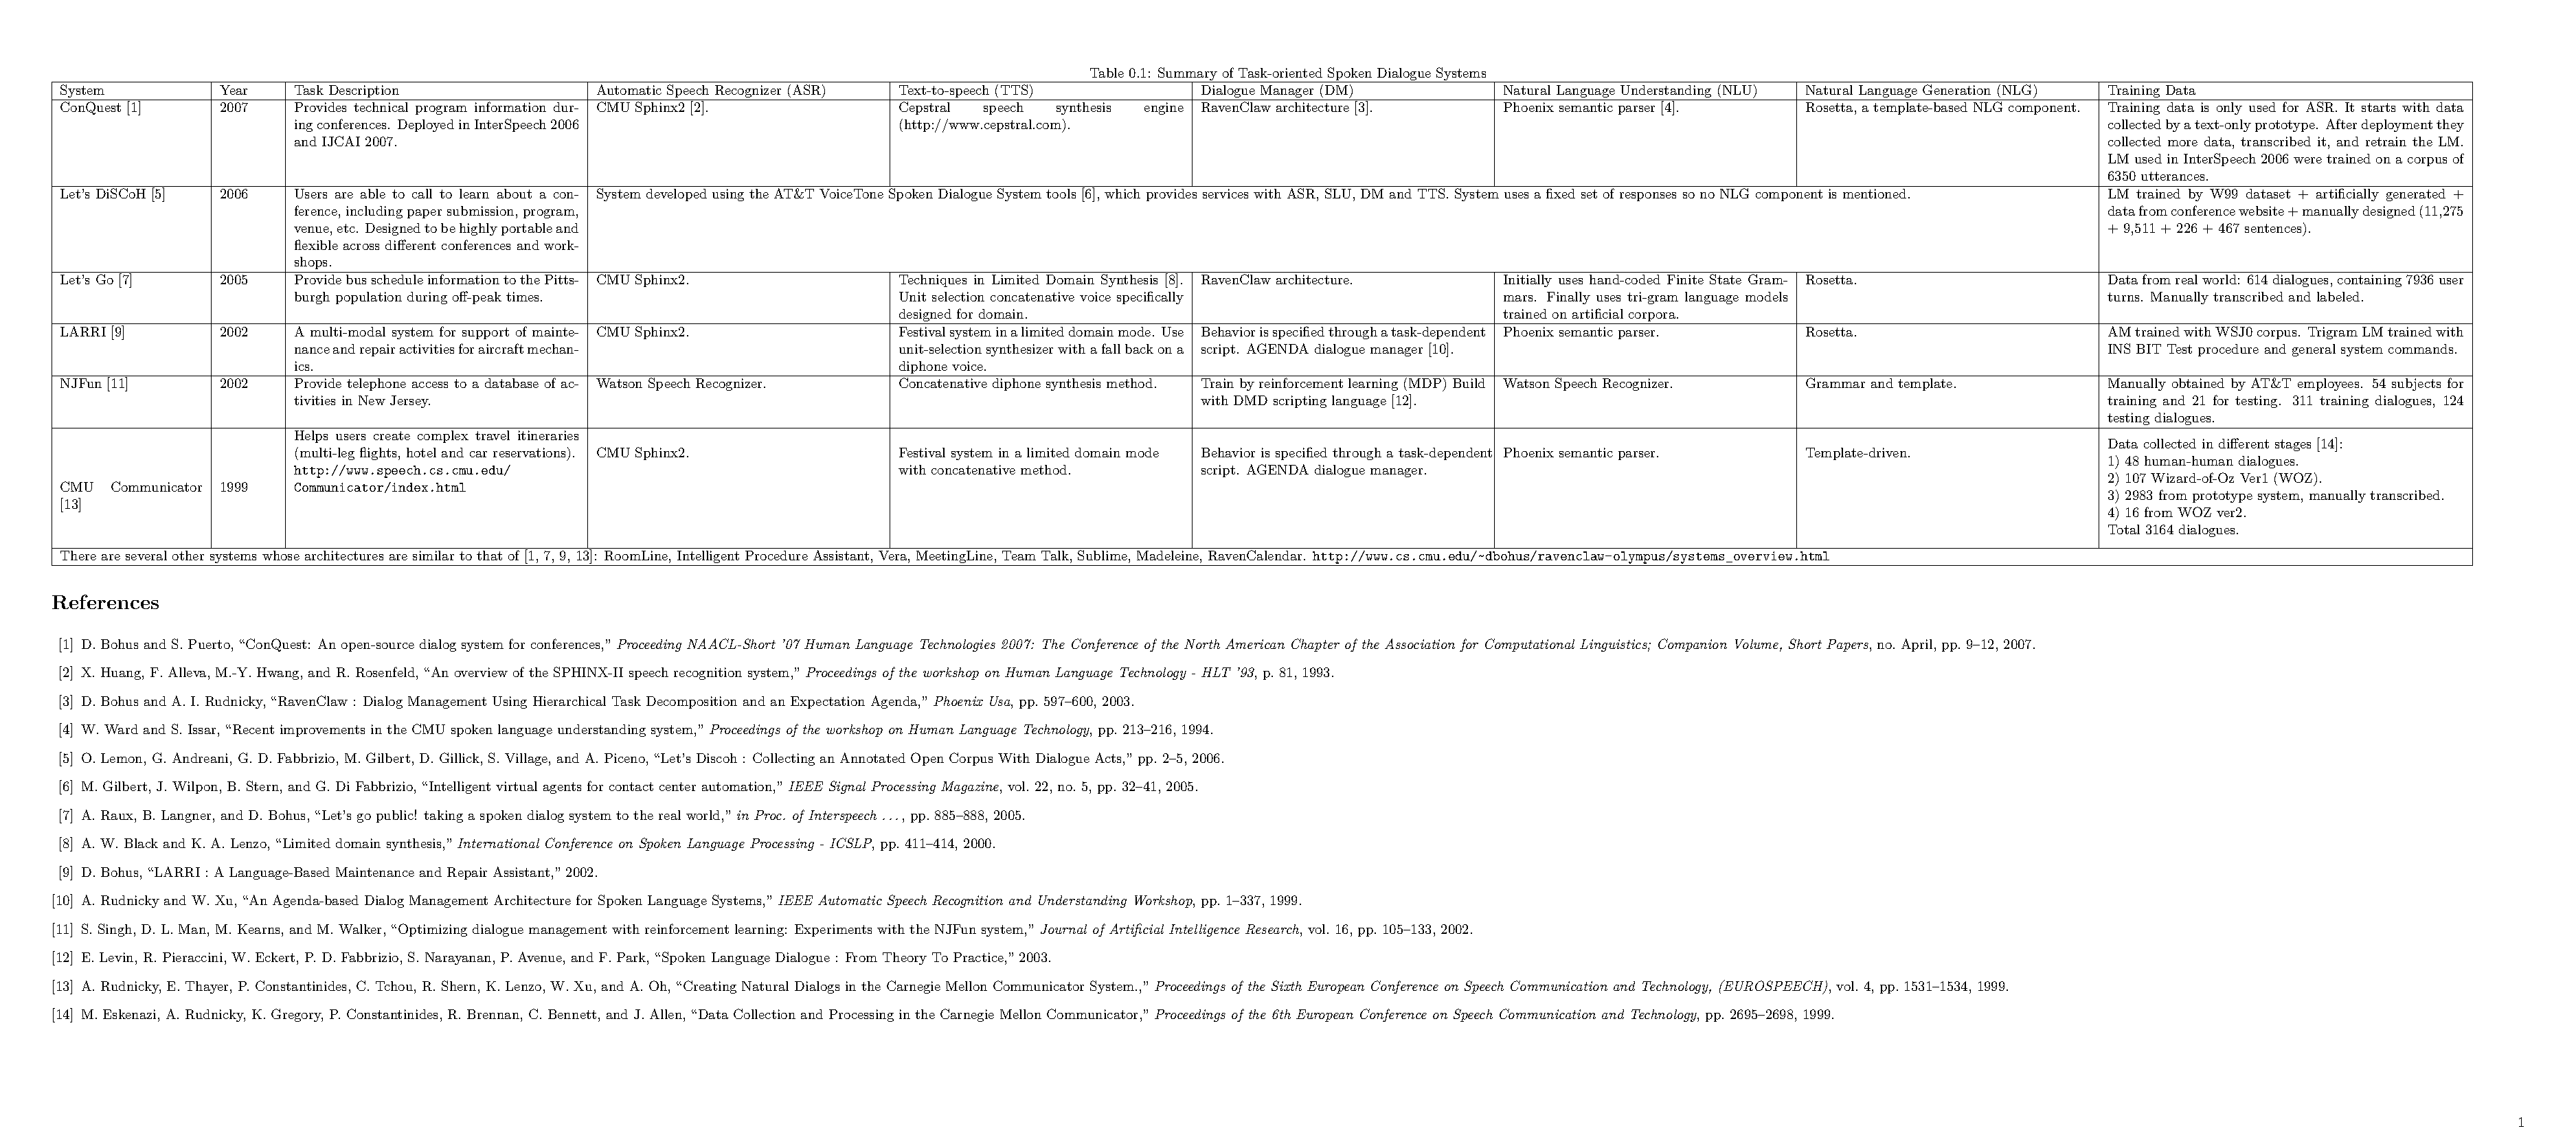
\includepdf[pages={-}, fitpaper=true]{docs/sys_table.pdf}
%\newpage

\bibliographystyle{ieeetr}
\bibliography{d:/research/chatbot}

\end{document}
